%███████╗ █████╗ ██████╗ ██╗███╗   ██╗ ██████╗ 
%██╔════╝██╔══██╗██╔══██╗██║████╗  ██║██╔════╝ 
%█████╗  ███████║██║  ██║██║██╔██╗ ██║██║  ███╗
%██╔══╝  ██╔══██║██║  ██║██║██║╚██╗██║██║   ██║
%██║     ██║  ██║██████╔╝██║██║ ╚████║╚██████╔╝
%╚═╝     ╚═╝  ╚═╝╚═════╝ ╚═╝╚═╝  ╚═══╝ ╚═════╝ 
%.:..:..:..:..:..:..:..:..:..:..:..:..:..:..:..:..:..:..:..:.
\section{Multi-path Fading}
Fading is the phenomenon that occurs when the amplitude and phase of a radio signal change rapidly over a short period of time or travel distance\cite{fuqin}.
Sky wave propagation, which involves passband transmitted signals being refracted by the ionosphere, tends to result in signals arriving at the receiver via different propagation paths and at varying time delays. These are \emph{multi-path components}.
These components have different carrier-phase offsets and may add destructively at times, resulting in fading\cite{Proakis}. 

The free space signal propagation model treats the region between the transmitting and receiving antennas as being free of obstacles. It also assumes that within the region, the atmosphere behaves as a uniform and non-absorbing medium. In this idealized model, the attenuation of \gls{RF} energy behaves according to an inverse square law\cite{AWGN}.
\[
	L_s(d) = \left( \frac{4\pi d}{\lambda} \right)^2
\]
\begin{mathDef}
	\mathSymb{d}{Distance from transmitter}
	\mathSymb{\lambda}{Wavelength of the propagating signal}
\end{mathDef}
For practical channels in which signal propagation takes place in the (non-uniform) atmosphere and close to the ground, the free space model is inadequate. Multi-path propagation causes fluctuations in the received signal's amplitude, phase and angle of arrival, all of which contribute to multi-path fading\cite{AWGN}.

In a multi-path channel, the received signal comprises a large number of plane waves whose complex low-pass signal can be modelled as a Gaussian random process\cite{fuqin}:
\[
	\tilde{r}(t) = r_I(t) + jr_Q(t)
\]
\begin{mathDef}
	\mathSymb{r}{Gaussian Random variable whose \(\mu = 0\) and \(\sigma^2 = 1\)}
\end{mathDef}

%,-.,-.,-.,-.,-.,-.,-.,-.,-.,-.,-.,-.,-.,-.,-.,-.,-.,-.,-.,-.
\subsection{Fading Channel Characteristics}
A fading channel is characterized by several parameters:
%`'`'`'`'`'`'`'`'`'`'
\paragraph{Delay Spread} In a multi-path channel, signal power at the receiver spreads over a certain period of time. The \(i\)\nth component's delay from the arrival of the 1st component is called \emph{excess delay}, denoted \(\tau_i\)\cite{fuqin}. Excess delay spread is defined as the longest time delay during which multi-path energy falls to X~dB below the maximum:
\[
	\tau_X - \tau_0
\]
\begin{mathDef}
	\mathSymb{\tau_0}{The delay of the first arriving signal component.}
	\mathSymb{\tau_X}{Maximum delay for which a component is within X~dB of the strongest.}
\end{mathDef}
The \emph{r.m.s. delay spread} \(\sqrt{\sigma_\tau}\) is the standard deviation of the delay of multi-path components, weighted proportional to their energy.
%`'`'`'`'`'`'`'`'`'`'
\paragraph{Coherence Bandwidth} This is the range of frequencies over which the channel can be considered frequency-flat\cite{Hindu} and can be determined using the reciprocal of delay spread\cite{Salehi}.
\[
	B_i = \frac{1}{\tau_i}
\]
%`'`'`'`'`'`'`'`'`'`'
\paragraph{Doppler Spread}
The \emph{Doppler spectrum} is the bandwidth of fluctuations of received signal strength. \emph{Doppler spread} \(B_D\) is a measure of spectrum broadening caused by relative movement of the mobile and base station or of obstacles on the ground.
\[
	B_D = f_M
\]
\begin{mathDef}
	\mathSymb{f_M}{Maximum Doppler Frequency}
\end{mathDef}
The total bandwidth of the received signal is determined by the bandwidth of the baseband signal and the Doppler spread. If baseband \(BW \gg B_D\) the effects of Doppler spread are negligible at the receiver.
%`'`'`'`'`'`'`'`'`'`'
\paragraph{Coherence Time}
This is the time interval between the arrival of the first and last multi-path components in a transmitted signal\cite{Hindu}.

%,-.,-.,-.,-.,-.,-.,-.,-.,-.,-.,-.,-.,-.,-.,-.,-.,-.,-.,-.,-.
\subsection{Channel Classification}
Fading channels are classified based on frequency-selectivity and coherence time:
%~^~~^~~^~~^~~^~~^~~^~~^~~^~~^~~^~~^~~^~~^~~^~~^~~^~~^~~^~~^~
\subsubsection{Flat fading}
This is also called \emph{non-frequency selective fading}. It is found in wireless channels with a constant gain and linear phase response over a bandwidth greater than signal bandwidth\cite{fuqin}. All of the received multi-path components of a symbol arrive within a single symbol duration. This means that the separate components are not resolvable.

There is no channel-induced \gls{ISI}. There is still performance degradation, as the unresolvable components may still add destructively to cause a significant reduction in \gls{SNR}. The fading channel is characterized by:
\begin{align*}
	B_c &> B_s \\
	\sigma_\tau &< T_s
\end{align*}
\begin{mathDef}
	\mathSymb{B_c}{Coherence Bandwidth}
	\mathSymb{B_s}{Signal Bandwidth}
	\mathSymb{T_s}{Symbol Duration}
\end{mathDef}
%~^~~^~~^~~^~~^~~^~~^~~^~~^~~^~~^~~^~~^~~^~~^~~^~~^~~^~~^~~^~
\subsubsection{Frequency Selective Fading}
A channel has frequency selective fading if multi-path delay time is greater than symbol time. The signal suffers \gls{ISI} due to time dispersion. Some frequency components have greater gains than others and thus the channel is considered a linear filter\cite{fuqin}. This channel is characterized by:
\begin{align*}
	B_c &< B_s \\
	\sigma_\tau &> T_s
\end{align*}
%~^~~^~~^~~^~~^~~^~~^~~^~~^~~^~~^~~^~~^~~^~~^~~^~~^~~^~~^~~^~
\subsubsection{Fast Fading}
This is a channel whose impulse response changes within a single symbol duration. Such rapid changes are attributed to motion or Doppler spreading. In fast fading, there is low data rate and high speed of the mobile unit\cite{fuqin}.

\noindent For a fast fading channel:
\begin{align*}
	T_s &> T_c \\
	B_s &< B_D
\end{align*}
%~^~~^~~^~~^~~^~~^~~^~~^~~^~~^~~^~~^~~^~~^~~^~~^~~^~~^~~^~~^~
\subsubsection{Slow Fading}
In slow fading, the channel impulse response changes at a slower rate than symbol rate. It corresponds to high data rate and low speed of the mobile unit. Characterized by:
\begin{align*}
	T_s &\ll T_c \\
	B_s &\gg B_D
\end{align*}

%,-.,-.,-.,-.,-.,-.,-.,-.,-.,-.,-.,-.,-.,-.,-.,-.,-.,-.,-.,-.
\subsection{Fading Envelope Distribution}
%~^~~^~~^~~^~~^~~^~~^~~^~~^~~^~~^~~^~~^~~^~~^~~^~~^~~^~~^~~^~
\subsubsection{Rayleigh Fading}
In a channel with a large number of reflective paths but no line-of-sight component, the received signal's envelope is statistically described by a Rayleigh \gls{PDF}\cite{AWGN}.

The Rayleigh distribution describes the statistical time-varying nature of the received envelope of a flat-fading signal\cite{4vn}. In considering a complex low-pass signal without a dominant multi-path component, \(r_I(t)\) and \(r_Q(t)\) are Gaussian processes with zero mean and a variance of \(\sigma^2\) \cite{fuqin}. The Rayleigh envelope \gls{PDF} is given by:
\begin{align*}
	p(z) &=
	\begin{cases}
		\frac{z}{\sigma^2} \exp \left( -\frac{z^2}{2\sigma^2} \right) & z \geq 0 \\
		0 & z < 0
	\end{cases}
\end{align*}
\begin{mathDef}
	\mathSymb{z}{Gaussian-distributed envelope magnitude}
\end{mathDef}
Maximum probability \(p(z)\) occurs at \(z=\sigma\):
\begin{figure}[!ht]
	\centering
	\resizebox{0.8\textwidth}{!}{\input{Graphics/LiteratureReview/rayleighPDF.pdf_tex}}
	\caption{Rayleigh probability distribution function}
\end{figure}
It is assumed that all multi-path components suffer the same attenuation but arrive at different phases, the amplitude corresponding to the Gaussian random variable \(z\)\cite{Hindu}.
%~^~~^~~^~~^~~^~~^~~^~~^~~^~~^~~^~~^~~^~~^~~^~~^~~^~~^~~^~~^~
\subsubsection{Rician Fading}
When there is a dominant (line-of-sight) propagation path, the fading envelope is described by a Rician \gls{PDF}\cite{AWGN}. Random multi-path components arrive at different angles and are superimposed on a stationary dominant signal. The \gls{PDF} of the Rician envelope is given by:
\begin{align*}
	p(z) =
	\begin{cases}
		\frac{z}{\sigma^2} \exp \left(-\frac{z^2 + A^2}{2\sigma^2}\right)I_0\left(\frac{Az}{\sigma^2}\right) & z \geq 0 \\
		0 & z < 0
	\end{cases}
\end{align*}
\begin{mathDef}
	\mathSymb{A}{Peak amplitude of the dominant signal.}
	\mathSymb{I_0(\cdot)}{0\nth\ modified Bessel function of the 1st kind\cite{fuqin}}
\end{mathDef}
\(K\) (in dB) is the ratio of the power of the specular signal to the power of the scattered components\cite{Hindu}.
\[
	K = 10 \log \frac{A^2}{2\sigma^2}
\]
Average power is given by:
\[
	E\{z^2\} = \Omega = A^2 + 2\sigma^2 = 2\sigma^2(1 + K)
\]
The Rician \gls{PDF} in terms of specular gain and average power:
\begin{align*}
	p(z) =
	\begin{cases}
		\frac{2z(K+1)}{\Omega} \exp \left(-K-\frac{(K+1)z^2}{\Omega}\right)I_0\left(2z\sqrt{\frac{K(K+1)}{\Omega}}\right) & z \geq 0 \\
		0 & z < 0
	\end{cases}
\end{align*}
The figure below shows the Rician distribution density for various \(K\) at fixed average power \(\Omega = 2\).
\begin{figure}[!h]
	\centering
	\resizebox{0.8\textwidth}{!}{\input{Graphics/LiteratureReview/riceanPDF.pdf_tex}}
	\caption{Rician probability distribution function}
\end{figure}

When \(A=0\) and therefore \(K=-\infty\), implying the absence of a specular component, the Rician distribution becomes a Rayleigh distribution.

%,-.,-.,-.,-.,-.,-.,-.,-.,-.,-.,-.,-.,-.,-.,-.,-.,-.,-.,-.,-.
\subsection{Q function}
The Gaussian \(Q\) function, or, equivalently, the error function \(\text{erf}(\cdot)\) is the tail distribution function of the standard normal distribution. \(Q(z)\) is defined as the probability that a normal random variable will obtain a value which is larger than \(z\) standard deviations\cite{qfuncber}.
The \(Q\) function is tabulated, and often made available as a built in function in mathematical software tools, for example as \texttt{qfunc(x)} in MATLAB.

The Gaussian process is the underlying model for an AWGN channel and its \gls{PDF} is given by:
\[
	p(x) = \frac{1}{\sigma \sqrt{2\pi}}e^{-\frac{(x-\mu)^2}{2\sigma^2}}
\]
\begin{mathDef}
	\mathSymb{\mu}{Population mean}
\end{mathDef}
\begin{figure}[!ht]
	\centering
	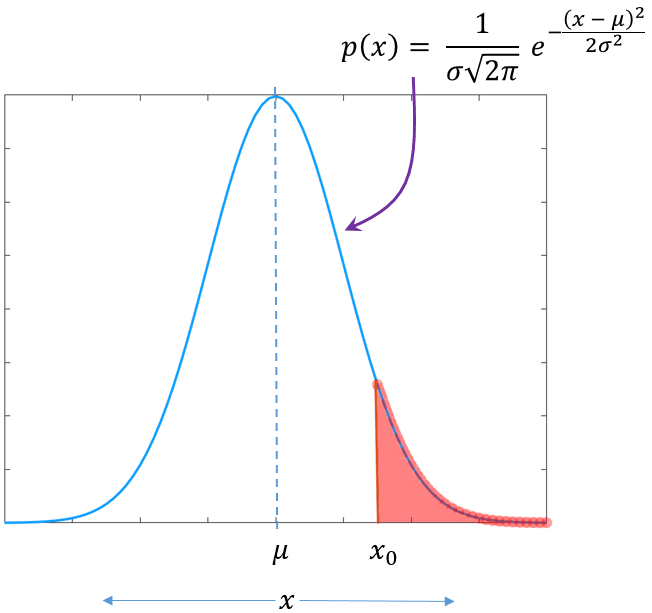
\includegraphics[scale=0.3]{Graphics/LiteratureReview/Qfunc.png}
	\caption{Gaussian PDF and Q function}
\end{figure}
The shaded region is evaluated as:
\[
	P(X \geq x_0) = \int_{x_0}^\infty \frac{1}{\sigma \sqrt{2\pi}}e^{-\frac{(x-\mu)^2}{2\sigma^2}}
\]
Substituting \(y = \frac{x - \mu}{\sigma}\), this can be re-written as:
\[
	P \left( y > \frac{x_0 - \mu}{\sigma}\right) = \int_{\frac{x_0 - \mu}{\sigma}}^{\infty} \frac{1}{\sqrt{2\pi}}e^{-\frac{y^2}{2}}dy
\]
The right-hand-side integral is termed as the \(Q\) function\cite{statistics}, given by:
\[
	Q(z) = \int_{\frac{x_0 - \mu}{\sigma}}^{\infty} \frac{1}{\sqrt{2\pi}}e^{-\frac{y^2}{2}}dy
\]
Thus the \(Q\) function gives the area of shaded part of the curve with the transformation \(y = \frac{x - \mu}{\sigma}\) applied to the Gaussian \gls{PDF}.

%,-.,-.,-.,-.,-.,-.,-.,-.,-.,-.,-.,-.,-.,-.,-.,-.,-.,-.,-.,-.
\subsection{Digital Modulation in slow, flat fading channels}
A signal undergoes multiplicative variation in a flat fading channel. This means that both amplitude and phase are affected since the multiplying coefficient is a complex one. In the worst case, amplitude attenuation and phase shift may be considered constant over a symbol duration. For a transmitted low-pass signal \(\tilde{s}(t)\), the received low-pass complex signal may be written as:
\[
	\tilde{r}(t) = ze^{-j\phi}\tilde{s}(t) + \tilde{n}(t)
\]
\begin{mathDef}
	\mathSymb{ze^{-j\phi}}{Complex channel gain}
	\mathSymb{\tilde{n}(t)}{Low-pass complex additive Gaussian noise.}
\end{mathDef}
The channel effect is corrected by dividing the received signal by the channel gain.
\[
	\tilde{r}_1(t) = \frac{\tilde{r}(t)}{ze^{-j\phi}} = \tilde{s}(t) + \frac{\tilde{n}(t)}{ze^{-j\phi}}
\]
Complex channel gain is estimated through \emph{equalization/channel estimation}.
